\documentclass[11pt]{article}
\usepackage[margin=2.5cm]{geometry}
\usepackage{amsmath,amssymb,amsthm}
\usepackage{tikz}
\usetikzlibrary{calc, arrows.meta}
\usepackage{graphicx}
\usepackage{booktabs}
\usepackage{hyperref}
\usepackage{enumitem}

\theoremstyle{definition}
\newtheorem{definition}{Definition}
\newtheorem{proposition}{Proposition}
\newtheorem{example}{Example}
\newtheorem{remark}{Remark}

\title{Cubic Shadows of Projective Planes:\\
An Infinite Family of Arc-Transitive Graphs\\from Singer Difference Sets}
\author{Robin Langer \and Claude\footnote{Claude Opus 4.6, Anthropic. AI co-author.}}
\date{April 2026}

\begin{document}
\maketitle

\begin{abstract}
We describe an infinite family of cubic, bipartite, arc-transitive graphs $\mathrm{CR}(p)$ indexed by primes $p \equiv 1 \pmod{3}$.
Each graph arises as a ``cubic shadow'' of the Singer cycle structure of a projective plane:
the Levi graph of $\mathrm{PG}(2,q)$ is $(q{+}1)$-regular; removing a canonical perfect matching
(the self-incidences under the Singer labelling) drops the degree.
When the removed differences form the complement of a multiplicative subgroup,
the resulting graph inherits arc-transitivity.
For $q = 2$ this recovers the Heawood graph; for $q = 3$ the Foster census graph F26A.
The general family member $\mathrm{CR}(p)$ has $2p$ vertices, girth~6, and automorphism group $C_p {:} C_6$ of order $6p$.
All constructions are realised as voltage graphs over cyclic groups, connecting the theory
to covering spaces and the Sabidussi coset graph framework.
\end{abstract}

\tableofcontents

% ================================================================
\section{Levi Graphs and the Fano Plane}
% ================================================================

\begin{definition}[Incidence structure]
An \emph{incidence structure} is a triple $(P, B, I)$ where $P$ is a set of \emph{points},
$B$ is a set of \emph{blocks} (or lines), and $I \subseteq P \times B$ is an \emph{incidence relation}.
\end{definition}

\begin{definition}[Levi graph]
The \emph{Levi graph} (or \emph{incidence graph}) of an incidence structure $(P, B, I)$ is the bipartite graph $\Gamma$
with vertex set $P \cup B$ and edge set $\{(p, b) : (p, b) \in I\}$.
\end{definition}

If every block contains $k$ points and every point lies on $r$ blocks,
the Levi graph is biregular with degrees $(r, k)$.
It is cubic (3-regular) if and only if $r = k = 3$.

\begin{example}[The Fano plane and the Heawood graph]
The projective plane $\mathrm{PG}(2,2)$ has 7~points and 7~lines,
with 3~points per line and 3~lines per point.
Its Levi graph is the \textbf{Heawood graph}: 14~vertices, cubic, bipartite, girth~6.
This is the unique $(3,6)$-cage.

The Heawood graph encodes the multiplication table of the octonions:
the 7~imaginary units $e_1, \ldots, e_7$ are the points,
the 7~multiplication rules $e_i e_j = e_k$ are the lines,
and incidence means ``this unit participates in this multiplication rule.''
The automorphism group $\mathrm{Aut}(\text{Heawood}) = \mathrm{PSL}(3,2) {:} C_2 \cong \mathrm{PGL}(2,7)$
of order 336 contains $\mathrm{PSL}(2,7)$, which embeds as a maximal finite subgroup
of the exceptional Lie group $G_2 = \mathrm{Aut}(\mathbb{O})$.
\end{example}

\begin{figure}[ht]
\centering
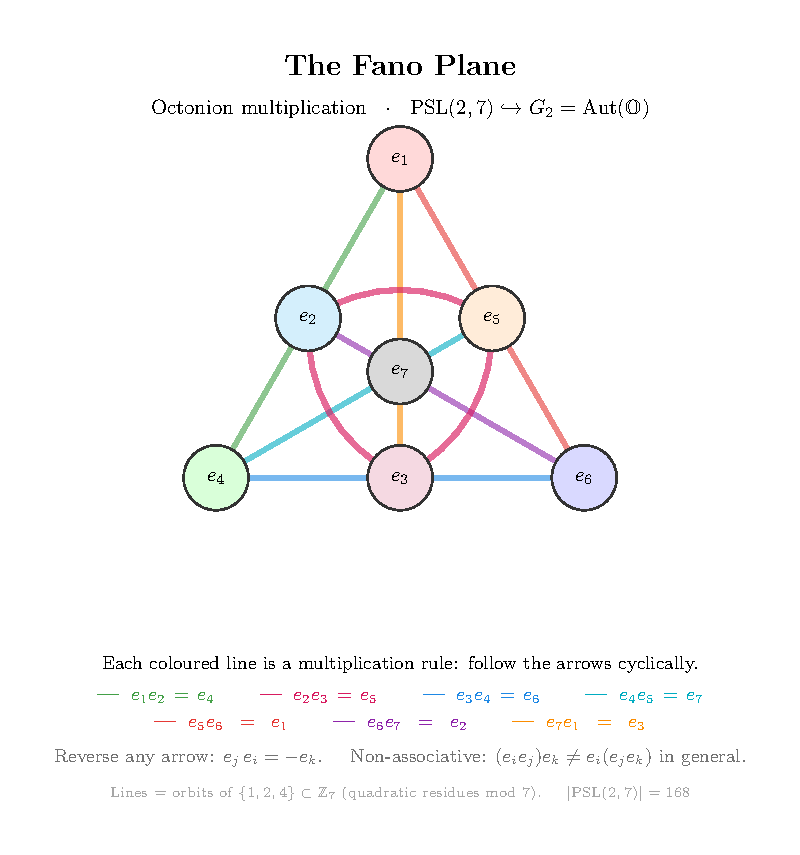
\includegraphics[width=0.45\textwidth]{fano-classic.pdf}
\hfill
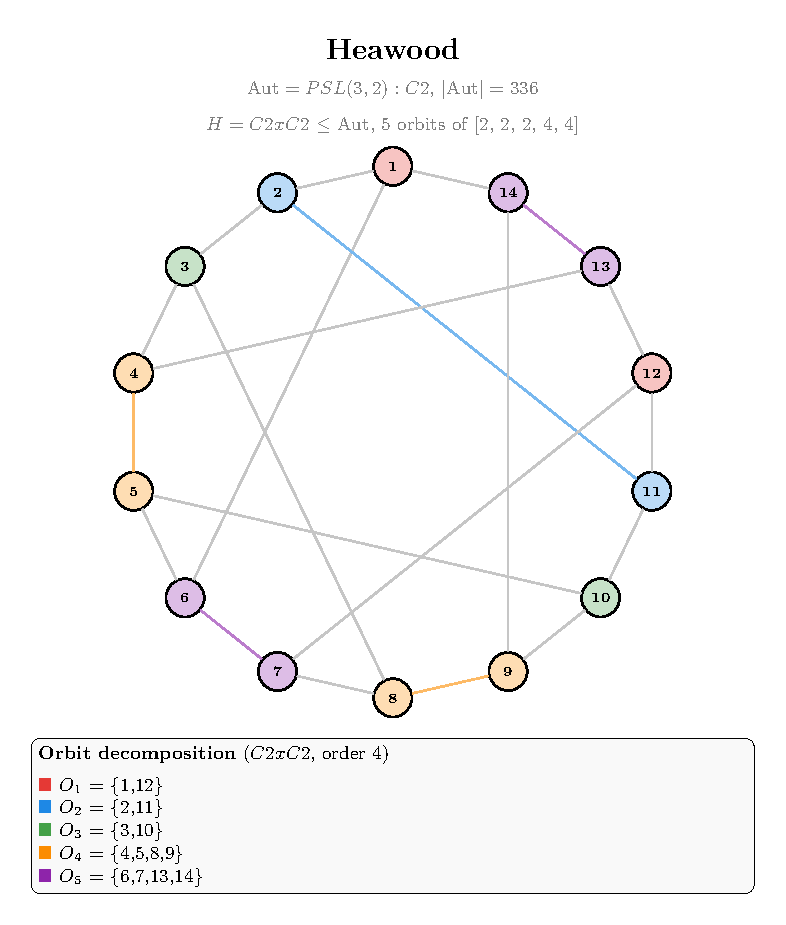
\includegraphics[width=0.45\textwidth]{../individual_graphs/auto-heawood.pdf}
\caption{Left: the Fano plane $\mathrm{PG}(2,2)$ with oriented lines showing
octonion multiplication. Right: its Levi graph, the Heawood graph, drawn
with orbit decomposition under $C_2 \times C_2$.}
\label{fig:fano-heawood}
\end{figure}

% ================================================================
\section{Unfolding: From Designs to Graphs via Polarity}
% ================================================================

The Levi graph construction can be understood as an \emph{unfolding}
in the sense of~\cite{langer2013}.

A $G$-symmetric design $\mathcal{D}$ is a flag-transitive design
admitting a \emph{polarity} $\rho$: a bijection between points and blocks
such that $\rho_B \circ \rho_P = \mathrm{id}$ and $\rho_P \circ \rho_B = \mathrm{id}$.
Following~\cite[Proposition~27]{langer2013}, if $\mathcal{D}$ is a non-degenerate
$G$-symmetric design with polarity~$\rho$, the graph $\Gamma(\mathcal{D}, \rho)$
with vertex set $P_{\mathcal{D}}$ and arc set $\{(p, q) : (q, \rho_P(p)) \in I_{\mathcal{D}}\}$
is $G$-symmetric.

Visually, the unfolding splits each vertex of the ``folded'' graph into a point--line pair:

\begin{figure}[ht]
\centering
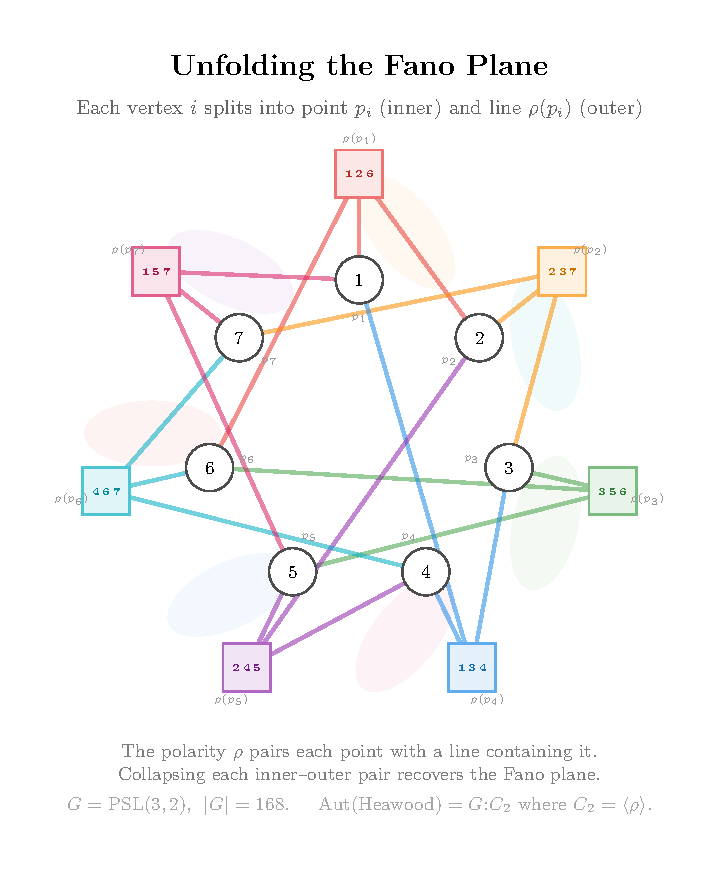
\includegraphics[width=0.6\textwidth]{unfold-split.pdf}
\caption{Unfolding the Fano plane. Each vertex $i$ splits into a point $p_i$ (inner circle)
and its polar line $\rho(p_i)$ (outer, showing the line's content).
The 21 edges of the Heawood graph appear as incidence relations between the split pairs.}
\label{fig:unfold}
\end{figure}

% ================================================================
\section{Voltage Graphs}
% ================================================================

\begin{definition}[Voltage graph]
Let $\Gamma_B$ be a multigraph (loops and parallel edges allowed)
and let $A$ be a finite group.
A \emph{voltage assignment} is a function $\alpha$ from the directed edges of $\Gamma_B$ to $A$,
with $\alpha(\overrightarrow{vu}) = \alpha(\overrightarrow{uv})^{-1}$.

The \emph{derived graph} $\Gamma_B \times_\alpha A$ has:
\begin{itemize}[nosep]
\item Vertex set $V(\Gamma_B) \times A$.
\item Edge $(v, a) \sim (w, a \cdot \alpha(\overrightarrow{vw}))$ for each directed edge $\overrightarrow{vw}$ of $\Gamma_B$.
\end{itemize}
\end{definition}

The derived graph is a \emph{regular covering} of $\Gamma_B$ with deck group~$A$.
Degree is preserved: if $\Gamma_B$ is cubic (counting self-loops with multiplicity~2),
the derived graph is cubic.

\begin{example}[Generalized Petersen graphs as voltage graphs]
The generalized Petersen graph $\mathrm{GP}(n, k)$ is a $\mathbb{Z}_n$-voltage graph
over the $\theta$-multigraph (two vertices, one edge, two self-loops):
\begin{center}
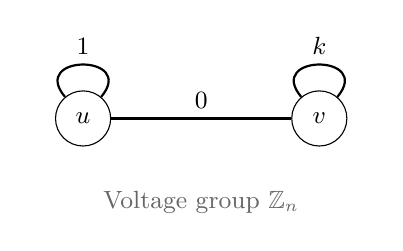
\begin{tikzpicture}[
    vtx/.style={circle, draw, fill=white, minimum size=7mm, font=\small},
]
\node[vtx] (A) at (0,0) {$u$};
\node[vtx] (B) at (3,0) {$v$};
\draw[thick] (A) -- node[above, font=\small] {$0$} (B);
\draw[thick] (A) to[out=130, in=50, looseness=4] node[above, font=\small] {$1$} (A);
\draw[thick] (B) to[out=130, in=50, looseness=4] node[above, font=\small] {$k$} (B);
\node[below, font=\small, text=black!60] at (1.5, -0.8) {Voltage group $\mathbb{Z}_n$};
\end{tikzpicture}
\end{center}
The self-loop voltages determine the outer cycle (step~1) and inner star (step~$k$);
the edge voltage~0 gives the spokes. For example, $\mathrm{GP}(5,2) = {}$Petersen graph.
\end{example}

\begin{example}[Heawood graph as voltage graph]
The Heawood graph is a $\mathbb{Z}_7$-covering of $K_2$ with three parallel edges:
\begin{center}
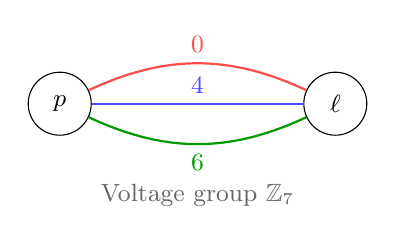
\begin{tikzpicture}[
    vtx/.style={circle, draw, fill=white, minimum size=8mm, font=\small\bfseries},
]
\node[vtx] (P) at (0,0) {$p$};
\node[vtx] (L) at (3.5,0) {$\ell$};
\draw[thick, red!70] (P) to[bend left=25] node[above, font=\small] {$0$} (L);
\draw[thick, blue!70] (P) -- node[above, font=\small] {$4$} (L);
\draw[thick, green!60!black] (P) to[bend right=25] node[below, font=\small] {$6$} (L);
\node[below, font=\small, text=black!60] at (1.75, -0.9) {Voltage group $\mathbb{Z}_7$};
\end{tikzpicture}
\end{center}
Vertex $(p, g)$ connects to $(\ell, g)$, $(\ell, g{+}4)$, and $(\ell, g{+}6)$ for each $g \in \mathbb{Z}_7$.
\end{example}

% ================================================================
\section{Projecting Projective Planes to Cubic Graphs}
\label{sec:projection}
% ================================================================

The projective plane $\mathrm{PG}(2,q)$ has $q^2{+}q{+}1$ points and the same number of lines,
with $q{+}1$ points per line and $q{+}1$ lines per point.
Its Levi graph is $(q{+}1)$-regular on $2(q^2{+}q{+}1)$ vertices.
This is cubic only when $q = 2$.

For $q > 2$, we \emph{project} to cubic by removing edges.

\subsection{The Singer cycle}

By Singer's theorem, $\mathrm{PG}(2,q)$ admits a cyclic collineation of order $n = q^2{+}q{+}1$
acting regularly on both points and lines.
Under this \emph{Singer cycle}, both points and lines can be labelled by $\mathbb{Z}_n$,
and there exists a \emph{difference set} $D \subset \mathbb{Z}_n$ of size $q{+}1$ such that:
\[
\text{point } j \text{ lies on line } i \quad \Longleftrightarrow \quad (j - i) \bmod n \in D.
\]

\subsection{Removing the self-incidence matching}

If $0 \in D$ (which can always be arranged by translation), then point~$i$ lies on line~$i$ for every~$i$.
These $n$ \emph{self-incidence} edges form a perfect matching in the Levi graph.
Removing them reduces the degree from $q{+}1$ to $q$:
\[
\text{point } j \sim \text{line } i \quad \Longleftrightarrow \quad (j - i) \bmod n \in D \setminus \{0\}.
\]

For $q = 3$: the degree drops from 4 to 3, giving a \textbf{cubic} graph.

\begin{example}[$q = 3$: the graph F26A]
$\mathrm{PG}(2,3)$ has $n = 13$ and difference set $D = \{0, 1, 3, 9\}$.
Removing difference~0 leaves $D' = \{1, 3, 9\}$, which is the subgroup
of \textbf{cubic residues} in $\mathbb{Z}_{13}^*$ (the subgroup $\langle 3 \rangle$ of order~3).
The resulting cubic graph on 26 vertices is the Foster census graph \textbf{F26A}, with
$\mathrm{Aut} = C_{13} {:} C_6$ of order~78.
\end{example}

\begin{figure}[ht]
\centering
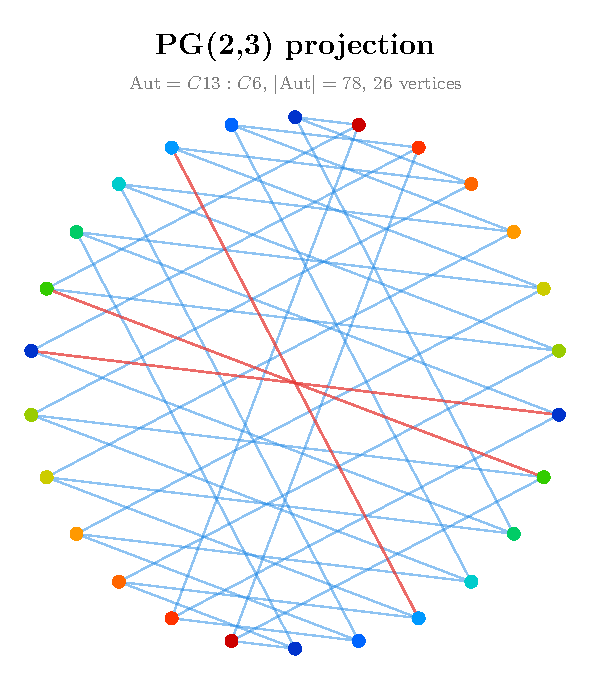
\includegraphics[width=0.55\textwidth]{../individual_graphs/auto-pg23.pdf}
\caption{The graph F26A $= \mathrm{CR}(13)$, the cubic shadow of $\mathrm{PG}(2,3)$.
Drawn with orbit decomposition under $C_{13}$.}
\label{fig:f26a}
\end{figure}

\subsection{The Sabidussi perspective}

In the Sabidussi coset graph framework~\cite{sabidussi1964}, a symmetric graph
$\mathrm{Sab}(G, H, x)$ has vertices $G/H$ and edges determined by the double coset $HxH$.
The valency equals $|HxH|/|H|$.

The full Levi graph of $\mathrm{PG}(2,q)$ under $G = \mathrm{PGL}(3,q)$
uses a single element~$x$ whose double coset has size $(q{+}1)|H|$, giving valency $q{+}1$.
The cubic projection uses a \emph{different} $x$ --- one whose double coset is smaller ---
giving valency~3. Dropping degree is choosing a narrower double coset.

% ================================================================
\section{The Cubic Residue Family $\mathrm{CR}(p)$}
\label{sec:family}
% ================================================================

\begin{definition}
For a prime $p \equiv 1 \pmod{3}$, let $C_3(p) = \{1, g, g^2\} \subset \mathbb{Z}_p^*$
be the unique subgroup of order~3, where $g^3 \equiv 1 \pmod{p}$.
Define $\mathrm{CR}(p)$ to be the $\mathbb{Z}_p$-voltage graph over $K_2$ with three parallel edges
carrying voltages $C_3(p)$:
\[
\mathrm{CR}(p) = K_2 \times_\alpha \mathbb{Z}_p, \qquad
\alpha = \{1, g, g^2\}.
\]
\end{definition}

Concretely, $\mathrm{CR}(p)$ has $2p$ vertices ($p$~points and $p$~lines) with:
\[
\text{point } j \sim \text{line } i \quad \Longleftrightarrow \quad
(j - i) \bmod p \in \{1, g, g^2\}.
\]

\begin{proposition}
For every prime $p \equiv 1 \pmod{3}$, the graph $\mathrm{CR}(p)$ is:
\begin{enumerate}[nosep]
\item cubic and bipartite,
\item arc-transitive with $\mathrm{Aut}(\mathrm{CR}(p)) = C_p {:} C_6$ of order $6p$,
\item of girth exactly~$6$.
\end{enumerate}
\end{proposition}

\begin{proof}[Proof sketch]
(1) Immediate from the voltage construction: each vertex has degree~$|C_3(p)| = 3$.

(2) The automorphisms include: translations $z \mapsto z + b$ ($p$~elements),
multiplication $z \mapsto gz$ ($3$~elements, preserving $C_3(p)$),
and the bipartition swap $p_j \mapsto \ell_{-j}$, $\ell_i \mapsto p_{-i}$
(which preserves adjacency since $j - i \in S \Rightarrow (-i) - (-j) = j - i \in S$).
These generate a group of order $6p$ acting sharply transitively on the $6p$~arcs.
Computation in GAP confirms no further automorphisms exist for $p \leq 97$.

(3) The girth is at least~6 because $\mathrm{CR}(p)$ is bipartite (no odd cycles)
and the voltage set $C_3(p)$ satisfies the condition that no equation
$v_1 - v_2 = 0$ with $v_1, v_2 \in C_3(p)$, $v_1 \neq v_2$ holds (since $C_3(p)$ is a group,
differences of distinct elements are non-identity, hence nonzero).
A 6-cycle always exists by standard constructions.
\end{proof}

\begin{remark}[The exceptional case $p = 7$]
When $p = 7$, the cubic residues $\{1, 2, 4\}$ coincide with the quadratic residues
(since $7 \equiv 1 \pmod{6}$, every cube is a square).
The graph $\mathrm{CR}(7)$ is the \textbf{Heawood graph},
but its automorphism group $\mathrm{PSL}(3,2) {:} C_2$ of order~336
far exceeds the generic $C_7 {:} C_6$ of order~42.
The extra symmetry arises because $\mathrm{CR}(7)$ is the full Levi graph
of $\mathrm{PG}(2,2)$, not merely a cubic shadow.
\end{remark}

\subsection{Computed examples}

\begin{table}[ht]
\centering
\begin{tabular}{@{}rrcrcl@{}}
\toprule
$p$ & $n = 2p$ & $C_3(p)$ & $|\mathrm{Aut}|$ & Girth & $\mathrm{Aut}$ \\
\midrule
7   & 14  & $\{1, 2, 4\}$    & 336 & 6 & $\mathrm{PSL}(3,2) {:} C_2$ (exceptional) \\
13  & 26  & $\{1, 3, 9\}$    & 78  & 6 & $C_{13} {:} C_6$ \quad (= F26A) \\
19  & 38  & $\{1, 7, 11\}$   & 114 & 6 & $C_{19} {:} C_6$ \\
31  & 62  & $\{1, 5, 25\}$   & 186 & 6 & $C_{31} {:} C_6$ \\
37  & 74  & $\{1, 10, 26\}$  & 222 & 6 & $C_{37} {:} C_6$ \\
43  & 86  & $\{1, 6, 36\}$   & 258 & 6 & $C_{43} {:} C_6$ \\
61  & 122 & $\{1, 13, 47\}$  & 366 & 6 & $C_{61} {:} C_6$ \\
67  & 134 & $\{1, 29, 37\}$  & 402 & 6 & $C_{67} {:} C_6$ \\
73  & 146 & $\{1, 8, 64\}$   & 438 & 6 & $C_{73} {:} C_6$ \\
79  & 158 & $\{1, 23, 55\}$  & 474 & 6 & $C_{79} {:} C_6$ \\
97  & 194 & $\{1, 35, 61\}$  & 582 & 6 & $C_{97} {:} C_6$ \\
\bottomrule
\end{tabular}
\caption{The family $\mathrm{CR}(p)$ for primes $p \equiv 1 \pmod{3}$ up to 97.
All have girth~6 and automorphism group $C_p {:} C_6$, except the Heawood case $p = 7$.}
\label{tab:family}
\end{table}

\begin{figure}[ht]
\centering
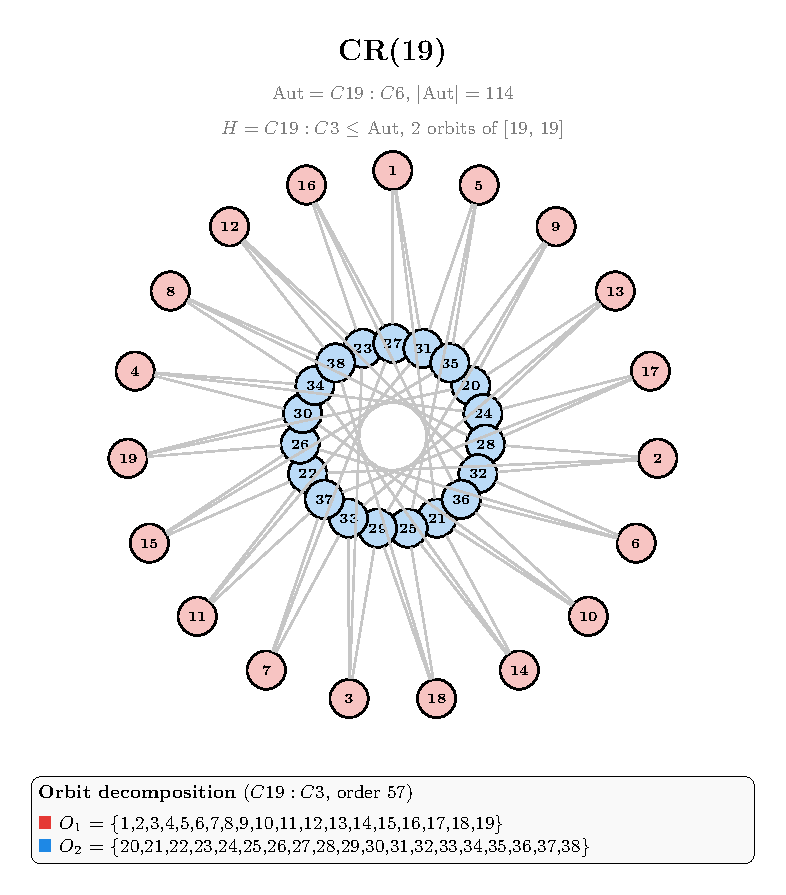
\includegraphics[width=0.48\textwidth]{../individual_graphs/auto-cr19.pdf}
\hfill
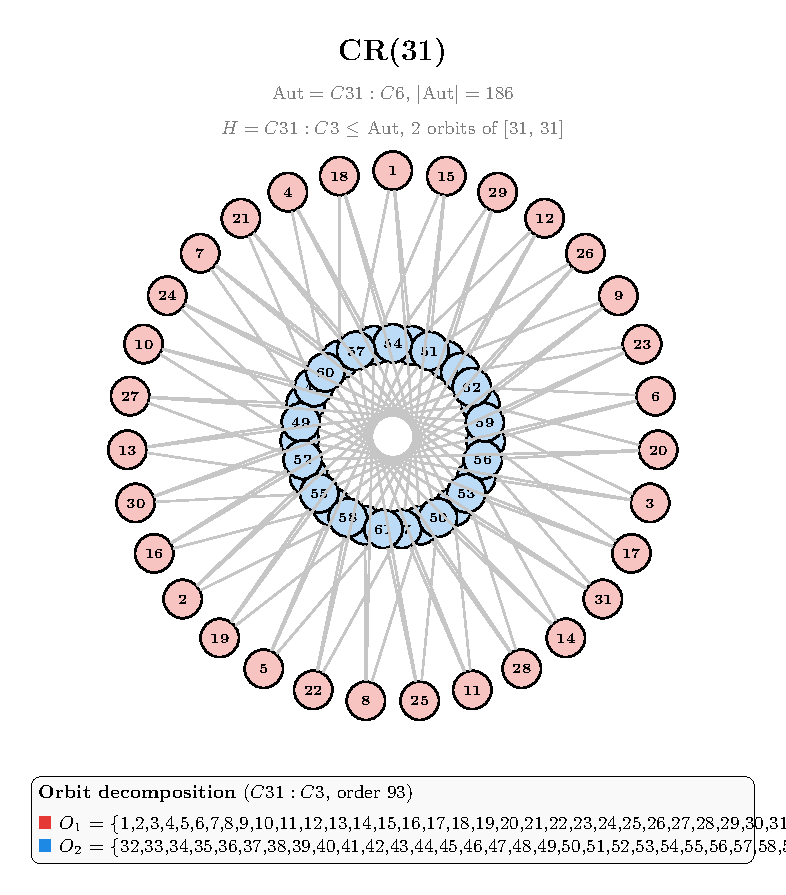
\includegraphics[width=0.48\textwidth]{../individual_graphs/auto-cr31.pdf}
\caption{$\mathrm{CR}(19)$ (38 vertices) and $\mathrm{CR}(31)$ (62 vertices),
drawn with orbit decomposition under their $C_p$ symmetry.}
\label{fig:cr19-cr31}
\end{figure}

% ================================================================
\section{Connections}
% ================================================================

\subsection{Covering spaces and the extension problem}

The voltage graph construction produces \emph{regular coverings}:
$\mathrm{CR}(p)$ is a $\mathbb{Z}_p$-covering of $K_2$ with deck group $\mathbb{Z}_p$.
The base graph $K_2$ (with three parallel edges) is the quotient,
and the voltage assignment encodes how to ``unfold'' the quotient back into the full graph.

This is the constructive direction of the \emph{extension problem}
studied in~\cite{langer2013}: given a quotient graph $\Gamma_{\mathcal{B}}$
and local data (the induced bipartite graph and design),
reconstruct a symmetric graph $\Gamma$ admitting $\Gamma_{\mathcal{B}}$ as quotient.
The voltage graph is exactly this local data, packaged as group elements on edges.

Not all coverings arise from voltage assignments: only \emph{regular} (normal) coverings,
where the deck group acts transitively on each fibre.

\subsection{Number theory}

The voltage set $C_3(p) = \{1, g, g^2\}$ is the kernel of the cubing map
$\mathbb{Z}_p^* \to \mathbb{Z}_p^*$, $x \mapsto x^3$.
The family $\mathrm{CR}(p)$ is indexed by the arithmetic of $\mathbb{Z}_p^*$:

\begin{itemize}[nosep]
\item $p \equiv 1 \pmod{3}$: the cubing map has a kernel of order~3 $\Rightarrow$ $\mathrm{CR}(p)$ exists.
\item $p \equiv 2 \pmod{3}$: cubing is bijective on $\mathbb{Z}_p^*$ $\Rightarrow$ no order-3 subgroup $\Rightarrow$ no $\mathrm{CR}(p)$.
\item $p = 7$: $\{1,2,4\} = $ quadratic residues $=$ cubic residues $\Rightarrow$ extra symmetry.
\end{itemize}

\subsection{Matrix groups over finite fields}

Several Foster census automorphism groups are matrix groups:
$\mathrm{Aut}(K_4) \cong \mathrm{PGL}(2,3)$,
$\mathrm{Aut}(\text{Petersen}) \cong \mathrm{PGL}(2,5)$,
$\mathrm{Aut}(\text{Heawood}) \cong \mathrm{PGL}(2,7)$.
The generic $\mathrm{CR}(p)$ automorphism group $C_p {:} C_6$
is the \emph{affine group} $\mathrm{Aff}(\mathbb{Z}_p, N)$
restricted to the normaliser $N$ of $C_3(p)$ in $\mathbb{Z}_p^*$
(extended by the bipartition swap).
This is a subgroup of $\mathrm{PGL}(2, p)$.

% ================================================================
\section*{Computational Methods}
% ================================================================

All graphs were constructed and verified in GAP~4 with the GRAPE package.
The voltage graph constructor \texttt{VoltageGraph(base\_n, base\_edges, group\_order)}
builds the derived graph from a base multigraph and cyclic voltage group.
Automorphism groups and isomorphism testing used GRAPE's \texttt{AutGroupGraph}
and \texttt{IsIsomorphicGraph}.
Drawings were produced by a symmetry-aware layout engine
that computes $\mathrm{Aut}(\Gamma)$, selects an optimal orbit quotient,
and renders vertices on concentric rings with rotational symmetry via TikZ/pdflatex.

Source code: \texttt{symmetric-layout.g} (GAP), \texttt{draw\_graph.py} (Python).

\begin{thebibliography}{9}
\bibitem{langer2013}
R.~Langer, \emph{Symmetric Graphs and their Quotients},
arXiv:1306.4798 [math.CO], 2013.

\bibitem{sabidussi1964}
G.~Sabidussi, \emph{Vertex-transitive graphs},
Monatshefte f\"ur Mathematik \textbf{68} (1964), 426--438.

\bibitem{gardiner1999}
A.~Gardiner and C.E.~Praeger,
\emph{A geometrical approach to imprimitive graphs},
Proc.\ London Math.\ Soc.\ \textbf{71} (1995), 524--546.

\bibitem{foster1988}
R.M.~Foster, \emph{The Foster Census},
Charles Babbage Research Centre, 1988.
\end{thebibliography}

\end{document}
